% !TEX root = ../Poissons.tex

\section{Combinatorics}

\subsection{Combinatorics of generically translated copies of the braid arrangement}
\label{sec:kBraidArrangement}

\subsubsection{Recollection on hyperplane arrangements}
\label{subsec:arrangements}

We first briefly recall classical results on the combinatorics of affine hyperplane arrangements, in particular the enumerative connection between their intersection posets and their face lattices due to T.~Zaslavsky~\cite{Zaslavsky}.

\begin{definition}
A (finite affine real) \defn{hyperplane arrangement} is a finite set~$\arrangement$ of affine hyperplanes in~$\R^d$.
\end{definition}

\begin{definition}
A \defn{region} of~$\arrangement$ is a connected component of~$\R^d \ssm \bigcup_{H \in \arrangement} H$.
A \defn{face} of~$\arrangement$ is the intersection of the closure of a region of~$\arrangement$ with an hyperplane of~$\arrangement$.
The \defn{face poset} of~$\arrangement$ is the poset~$\facePoset$ of faces of~$\arrangement$ ordered by inclusion.
The \defn{$f$-polynomial}~$\fPol$ and \defn{$b$-polynomial}~$\bPol$ of~$\arrangement$ are the polynomial
\[
\fPol \eqdef \sum_{k = 0}^d f_k(\arrangement) \, x^k
\qquad\text{and}\qquad
\bPol \eqdef \sum_{k = 0}^d b_k(\arrangement) \, x^k
\]
where~$f_k(\arrangement)$ denotes the number of $k$-dimensional faces of~$\arrangement$, while~$b_k(\arrangement)$ denotes the number of bounded $k$-dimensional faces of~$\arrangement$.
\end{definition}

\begin{definition}
A \defn{flat} of~$\arrangement$ is a non-empty affine subspace of~$\R^d$ that can be obtained as the intersection of some hyperplanes of~$\arrangement$.
The \defn{flat poset} of~$\arrangement$ is poset~$\flatPoset$ of flats of~$\arrangement$ ordered by reverse inclusion.
\end{definition}

\begin{definition}
%The \defn{characteristic polynomial}~$\chi_{\arrangement}(y)$ and the \defn{M\"obius polynomial}~$\mu_{\arrangement}(x,y)$ are the polynomials respectively defined by
%\[
%\charPol \eqdef \sum_{G \in \flatPoset} \mu_{\flatPoset}(\R^d, G) \, y^{\dim(G)}
%\quad\text{and}\quad
%\mobPol \eqdef \sum_{F \le G \in \flatPoset} \mu_{\flatPoset}(F,G) \, x^{\dim(F)} \, y^{\dim(G)}
%\]
The \defn{M\"obius polynomial}~$\mu_{\arrangement}(x,y)$ is the polynomial defined by
\[
\mobPol \eqdef \sum_{F \le G} \mu_{\flatPoset}(F,G) \, x^{\dim(F)} \, y^{\dim(G)},
\]
where~$F \le G$ ranges over all intervals of the flat poset~$\flatPoset$, and~$\mu_{\flatPoset}(F,G)$ denotes the \defn{M\"obius function} on the flat poset~$\flatPoset$ defined as usual by
\[
\mu_{\flatPoset}(F, F) = 1
\qquad\text{and}\qquad
\sum_{F \le G \le H} \mu_{\flatPoset}(F,G) = 0
\]
for all~$F, G, H \in \flatPoset$.
\vincent{Whitney-number polynomial.}
\vincent{Note that this is not the M\"obius polynomial defined by Zaslavsky. I decided to take the dimension instead of the codimension.}
\end{definition}

\begin{theorem}[{\cite[Thm.~A]{Zaslavsky}}]
The $f$-polynomial, the $b$-polynomial, and the M\"obius polynomial of an arrangement~$\arrangement$ are related by
\[
\fPol = (-1)^{\rank} \mobPol[\arrangement][-x][-1]
\qquad\text{and}\qquad
\bPol = (-1)^{\rank} \mobPol[\arrangement][-x][1].
\]
\end{theorem}

\vincent{Whitney's theorem?}

\begin{example}
For the arrangement~$\arrangement$ of $5$ hyperplanes of \cref{fig:arrangement}, we have
\[
\mobPol = x^2y^2 - 5x^2y + 6x^2 + 5xy - 10x + 4
\]
so that
\begin{align*}
\fPol & = \mobPol(-x,-1) = 12 \, x^2 + 15 \, x + 4 \\
\text{and}\qquad
\bPol & = \mobPol(-x,1) = 2 \, x^2 + 5 \, x + 4.
\end{align*}
%
\begin{figure}
%	\begin{overpic}[scale=.9]{intersectionPoset}
%		\put(72.5, -2){$1$}
%		\put(51, 10){$-1$}
%		\put(61, 10){$-1$}
%		\put(71, 10){$-1$}
%		\put(82, 10){$-1$}
%		\put(94, 10){$-1$}
%		\put(51.5, 32){$2$}
%		\put(66, 32){$1$}
%		\put(80, 32){$1$}
%		\put(93.5, 32){$2$}
%	\end{overpic}
%	\caption{A hyperplane arrangement (left) and its intersection poset with its M\"obius function (right).}
	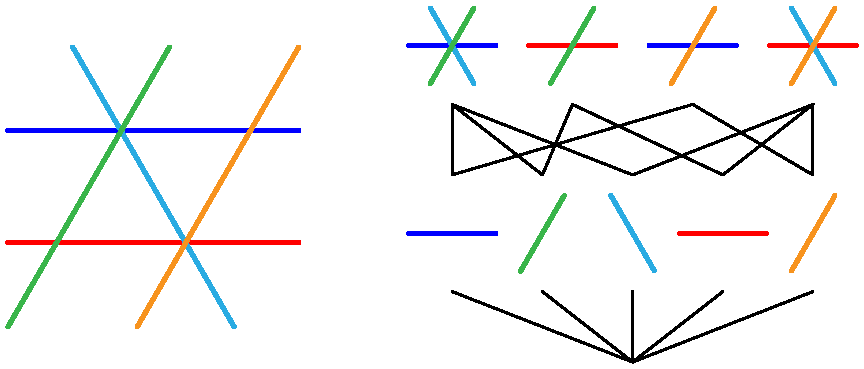
\includegraphics[scale=.9]{intersectionPoset}
	\caption{A hyperplane arrangement (left) and its intersection poset (right).}
	\label{fig:arrangement}
\end{figure}
\end{example}

\subsubsection{The $(\ell,n)$-braid arrrangement}
\label{subsec:lnBraidArrangement}

We now focus on the following specific hyperplane arrangements, illustrated in \cref{fig:lBraidArrangements}, and whose face numbers are given in \cref{table:fvectorlBraidArrangements}.

\begin{figure}
	\centerline{
	\begin{tabular}{c@{\hspace{.7cm}}c@{\hspace{.7cm}}c@{\hspace{.7cm}}c}
		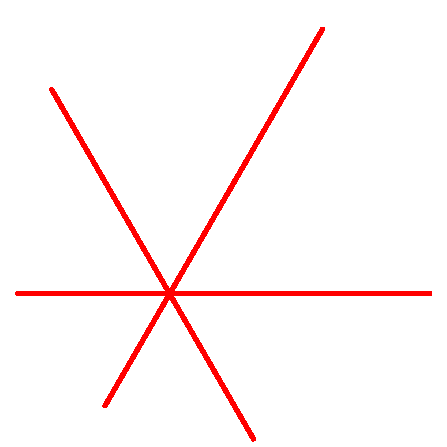
\includegraphics[scale=.4]{lBraidArrangement1}
		&
		\includegraphics[scale=.4]{lBraidArrangement2}
		&
		\includegraphics[scale=.4]{lBraidArrangement3}
		&
		\includegraphics[scale=.4]{lBraidArrangement4}
		\\
		$\ell = 1$ & $\ell = 2$ & $\ell = 3$ & $\ell = 4$
	\end{tabular}
	}
	\caption{The $(\ell,3)$-braid arrangements for~$\ell \in [4]$.}
	\label{fig:lBraidArrangements}
\end{figure}

\begin{table}
\centerline{
	\begin{tabular}{c@{\hspace{.7cm}}c@{\hspace{.7cm}}c@{\hspace{.7cm}}c}
		\begin{tabular}[t]{c|cccc|c}
			$n \backslash k$ & $0$ & $1$ & $2$ & $3$ & $\Sigma$ \\
			\hline
			$1$ & $1$ &&&& $1$ \\
			$2$ & $2$ & $1$ &&& $3$ \\
			$3$ & $6$ & $6$ & $1$ && $13$ \\
			$4$ & $24$ & $36$ & $14$ & $1$ & $75$
		\end{tabular}
		&
		\begin{tabular}[t]{c|cccc|c}
			$n \backslash k$ & $0$ & $1$ & $2$ & $3$ & $\Sigma$ \\
			\hline
			$1$ & $1$ &&&& $1$ \\
			$2$ & $3$ & $2$ &&& $5$ \\
			$3$ & $17$ & $24$ & $8$ && $49$ \\
			$4$ & $149$ & $324$ & $226$ & $50$ & $749$
		\end{tabular}
		&
		\begin{tabular}[t]{c|cccc|c}
			$n \backslash k$ & $0$ & $1$ & $2$ & $3$ & $\Sigma$ \\
			\hline
			$1$ & $1$ &&&& $1$ \\
			$2$ & $4$ & $3$ &&& $7$ \\
			$3$ & $34$ & $54$ & $21$ && $109$ \\
			$4$ & $472$ & $1152$ & $924$ & $243$ & $2791$
		\end{tabular}
		&
		\begin{tabular}[t]{c|cccc|c}
			$n \backslash k$ & $0$ & $1$ & $2$ & $3$ & $\Sigma$ \\
			\hline
			$1$ & $1$ &&&& $1$ \\
			$2$ & $5$ & $4$ &&& $9$ \\
			$3$ & $57$ & $96$ & $40$ && $193$ \\
			$4$ & $1089$ & $2808$ & $2396$ & $676$ & $6969$
		\end{tabular}
		\\[2cm]
		\begin{tabular}[t]{c|cccc|c}
			$n \backslash k$ & $0$ & $1$ & $2$ & $3$ & $\Sigma$ \\
			\hline
			$1$ & $1$ &&&& $1$ \\
			$2$ & $0$ & $1$ &&& $1$ \\
			$3$ & $0$ & $0$ & $1$ && $1$ \\
			$4$ & $0$ & $0$ & $0$ & $1$ & $1$
		\end{tabular}
		&
		\begin{tabular}[t]{c|cccc|c}
			$n \backslash k$ & $0$ & $1$ & $2$ & $3$ & $\Sigma$ \\
			\hline
			$1$ & $1$ &&&& $1$ \\
			$2$ & $1$ & $2$ &&& $3$ \\
			$3$ & $5$ & $12$ & $8$ && $25$ \\
			$4$ & $43$ & $132$ & $138$ & $50$ & $363$
		\end{tabular}
		&
		\begin{tabular}[t]{c|cccc|c}
			$n \backslash k$ & $0$ & $1$ & $2$ & $3$ & $\Sigma$ \\
			\hline
			$1$ & $1$ &&&& $1$ \\
			$2$ & $2$ & $3$ &&& $5$ \\
			$3$ & $16$ & $36$ & $21$ && $73$ \\
			$4$ & $224$ & $684$ & $702$ & $243$ & $1853$
		\end{tabular}
		&
		\begin{tabular}[t]{c|cccc|c}
			$n \backslash k$ & $0$ & $1$ & $2$ & $3$ & $\Sigma$ \\
			\hline
			$1$ & $1$ &&&& $1$ \\
			$2$ & $3$ & $4$ &&& $7$ \\
			$3$ & $33$ & $72$ & $40$ && $145$ \\
			$4$ & $639$ & $1944$ & $1980$ & $676$ & $5239$
		\end{tabular}
		\\[2cm]
		$\ell = 1$ & $\ell = 2$ & $\ell = 3$ & $\ell = 4$
	\end{tabular}
	}
	\vspace{.3cm}
	\caption{The face numbers (top) and the bounded face numbers (bottom) of the $(\ell,n)$-braid arrangements for~$\ell, n \in [4]$.}
	\label{table:fvectorlBraidArrangements}
\end{table}

\vincent{I still have to decide what I do with this big \cref{table:fvectorlBraidArrangements}.}

\begin{definition}
For any integer~$\ell 1$, the \defn{braid arrangement}~$\braidArrangement$ is the arrangement of the hyperplanes~$\set{\b{x} \in \R^n}{x_i = x_j}$ for all~$1 \le i < j \le n$.
For any integer~$\ell 1$, the \defn{$(\ell,n)$-braid arrangement}~$\lBraidArrangement$ is the arrangement obtained as the union of $\ell$ generically translated copies of the braid arrangement.
\end{definition}

\begin{remark}[Combinatorics of the braid arrangement]
\vincent{TODO. Partitions, refinement poset on partitions, M\"obius function given by~$(-1)^{p-1} (p-1)!$.}
\end{remark}

\begin{definition}
The \defn{intersection hypergraph}~$I(F_1, \dots, F_\ell)$ of a $\ell$-tuple of partitions of~$[n]$ is the $\ell$-regular $\ell$-partite hypergraph on all parts of all the partitions~$F_i$, with an hyperedge for all~$i \in [n]$ connecting the parts containing~$i$.
A \defn{$(\ell,n)$-forest} (resp.~\defn{$(\ell,n)$-tree}) is a $\ell$-tuple~$\b{F} \eqdef (F_1, \dots, F_\ell)$ of partitions of~$[n]$ whose intersection hypergraph is a hyperforest (resp.~hypertree).
See \cref{fig:forests}.
The \defn{$(\ell,n)$-forest poset} is the poset~$\forestPoset$ on $(\ell,n)$-forests ordered by componentwise refinement.
In other words, $\forestPoset$ is the subposet of the $\ell$th Cartesian power of the partition poset induced by $(\ell,n)$-forests.
%
\begin{figure}
	\centerline{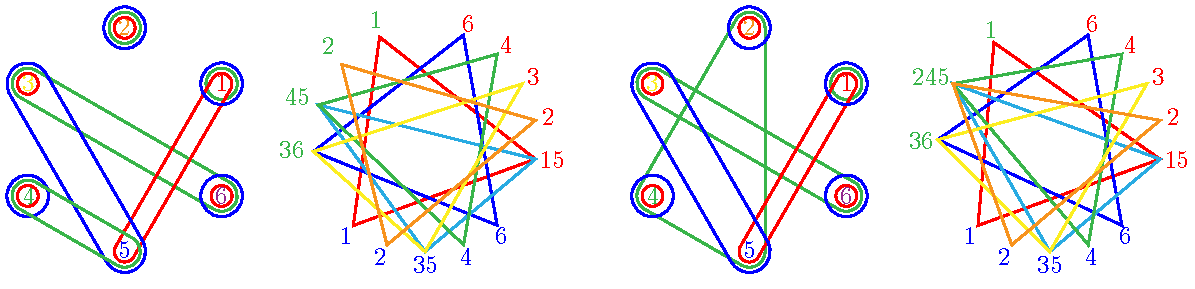
\includegraphics[scale=1]{forests}}
	\caption{A $(3,6)$-forest with its intersection hypergraph (left) and a $(3,6)$-tree with its intersection hypergraph (right).}
	\label{fig:forests}
\end{figure}
\end{definition}

\begin{theorem}
\label{thm:MobiusPolynomial}
The M\"obius polynomial of the $(\ell,n)$-braid arrangement~$\lBraidArrangement$ is given by
\[
\mobPol[\lBraidArrangement] = \sum_{\b{F} \le \b{G}} \prod_{i \in [\ell]} x^{\#F_i-1} y^{\#G_i-1} \prod_{p \in G_i} (-1)^{\#F_i[p]-1} (\# F_i[p]-1)! \; ,
\]
where~$\b{F} \le \b{G}$ ranges over all intervals of the $(\ell,n)$-forest poset~$\forestPoset$, and~$F_i[p]$ denotes the restriction of the partition~$F_i$ to the part~$p$ of~$G_i$.
\end{theorem}

\begin{proof}
Observe that for~$\b{F} = (F_1, \dots, F_\ell)$ and~$\b{G} = (G_1, \dots, G_\ell)$ in~$\forestPoset$, we have
\[
[\b{F}, \b{G}] = \prod_{i \in [\ell]} [F_i, G_i] \simeq \prod_{i \in [\ell]} \prod_{p \in G_i} \partitionPoset[{\#F_i[p]}].
\]
As the M\"obius function is multiplicative, that is,
\(
\mu_{P \times Q} \big( (p,q), (p’,q’) \big) = \mu_P(p,p’) \cdot \mu_Q(q,q’),
\)
we obtain that
\[
\mu_{\forestPoset}(\b{F}, \b{G}) = \prod_{i \in [\ell]} \prod_{p \in G_i} (-1)^{\#F_i[p]-1} (\# F_i[p]-1)!
\]
Hence
\begin{align*}
\mobPol[\lBraidArrangement] 
& = \sum_{\b{F} \le \b{G}} \mu_{\forestPoset}(\b{F}, \b{G}) \, x^{\dim(\b{F})} \, y^{\dim(\b{G})} \\
% & = \sum_{\b{F} \le \b{G}} \prod_{i \in [\ell]} x^{\#F_i-1} y^{\#G_i-1} \\
& = \sum_{\b{F} \le \b{G}} \prod_{i \in [\ell]} x^{\#F_i-1} y^{\#G_i-1} \prod_{p \in G_i} (-1)^{\#F_i[p]-1} (\# F_i[p]-1)!.
\qedhere
\end{align*}
\end{proof}

\begin{corollary}
The $f$- and $b$-polynomials of the $(\ell,n)$-braid arrangement~$\lBraidArrangement$ are given by
\begin{align*}
\fPol[\lBraidArrangement] & = \sum_{\b{F} \le \b{G}} \prod_{i \in [\ell]} x^{\#F_i-1} \prod_{p \in G_i} (\# F_i[p]-1)!\\
\text{and}\qquad
\bPol[\lBraidArrangement] & = (-1)^\ell \sum_{\b{F} \le \b{G}} \prod_{i \in [\ell]} x^{\#F_i-1} \prod_{p \in G_i} -(\# F_i[p]-1)!
\end{align*}
\end{corollary}

The face numbers and bounded face numbers of~$\lBraidArrangement$ for~$\ell, n \in [4]$ are gathered in \cref{table:fvectorlBraidArrangements}.

\begin{example}[$n \le 3$]
For~$n = 1$, we have
\[
\mobPol[{\lBraidArrangement[1][\ell]}] = \fPol[{\lBraidArrangement[1][\ell]}] = \bPol[{\lBraidArrangement[1][\ell]}] = 1.
\]
For~$n = 2$, we have
\[
\mobPol[{\lBraidArrangement[2][\ell]}] = xy-\ell x+\ell,
\quad
\fPol[{\lBraidArrangement[2][\ell]}] = (\ell+1)x+\ell
\quad\text{and}\quad
\bPol[{\lBraidArrangement[2][\ell]}] = (\ell-1)x+\ell.
\]
The case~$n = 3$ is already more interesting.
\vincent{Explain here the $(\ell,3)$-forests.}
Hence, we have
\begin{align*}
\mobPol[{\lBraidArrangement[3][\ell]}] & = x^2 y^2 - 3 \ell x^2 y + \ell (3 \ell - 1) x^2 + 3 \ell x y - 3 \ell (2 \ell - 1) x + \ell (3 \ell - 2) , \\
\fPol[{\lBraidArrangement[3][\ell]}] & = (3 \ell^2 + 2 \ell + 1) x^2 + 6 \ell^2 x + \ell (3 \ell - 2) \\
\text{and}\qquad
\bPol[{\lBraidArrangement[3][\ell]}] & = (3 \ell^2 - 4 \ell + 1) x^2 + 6 \ell (\ell - 1) x + \ell (3 \ell - 2).
\end{align*}
Note that~$3 \ell^2 + 2 \ell + 1$ is~\OEIS{A056109}, that~$\ell (3 \ell - 2)$ is~\OEIS{A000567}, and that~$3 \ell^2 - 4 \ell + 1$ is~\OEIS{A045944}.
\vincent{There is a weird connection between the first and the last. Namely, $3 \ell^2 - 4 \ell + 1 = 3 (\ell - 1)^2 + 2 (\ell - 1)$. Is there a bijective explanation on the arrangements?}
\end{example}

\begin{theorem}
Number of vertices.
\vincent{Berenice, the floor is yours...}
\end{theorem}

\subsection{Enumerative results for any diagonal} 
\label{s:facets}

We now specialize the results of the previous section to the case~$\ell = 2$ to derive enumerative results on the diagonal of the permutahedron.
\vincent{TODO. Nice bijection for vertices. Generating functions for facets and bounded facets.}

